% Module 2: Tasks in Medical Image Analysis -- How to Train a CNN
% Companion deck to main.tex (Module 1). Reuses styles/, loadslides.tex, Figures/.
% Style block below is copied from main.tex (Module 1) so main.tex is left untouched.

\documentclass[
11pt,notheorems,hyperref={pdfauthor=whatever}
]{beamer}

\usepackage{amssymb}
\usepackage{tcolorbox}
\usepackage{graphicx}
\usepackage{xcolor}
\renewcommand{\familydefault}{\sfdefault}
\usepackage{tikz}
\usepackage{tikz-3dplot}
\usetikzlibrary{positioning, arrows.meta, shapes.geometric, calc, backgrounds, fit}

\input{loadslides.tex} % Loads packages and some defined commands (elegant theme, \makepart)
\setbeamertemplate{footline}{}
\setbeamersize{
  text margin left=60mm,
  text margin right=10mm
}

% put these AFTER the theme/colors are loaded
\setbeamercolor{background canvas}{bg=black}
\setbeamercolor{normal text}{fg=white,bg=black}

% --- Accent + background palette (shared with Module 1) ---
\definecolor{accTeal}{RGB}{77, 208, 225}
\definecolor{accGreen}{RGB}{129, 199, 132}
\definecolor{accAmber}{RGB}{255, 213, 79}
\definecolor{accCoral}{RGB}{255, 138, 101}

\definecolor{bgTeal}{RGB}{15, 30, 40}
\definecolor{bgGreen}{RGB}{15, 30, 20}
\definecolor{bgAmber}{RGB}{30, 25, 10}
\definecolor{bgCoral}{RGB}{35, 15, 15}

% accent color used in Module 1's Classification part (kept for continuity)
\definecolor{accent}{HTML}{00D4FF}
\definecolor{softblue}{HTML}{5E7BFF}
\definecolor{labelgreen}{HTML}{7CFF8A}

\newcommand{\HUGE}{\fontsize{28pt}{32pt}\selectfont}
\newcommand{\boximageWide}[1]{%
    \begin{minipage}[c][7.2cm][c]{7cm}
        \centering
        \includegraphics[width=7cm, height=7.2cm, keepaspectratio]{Figures/#1}
    \end{minipage}\par\vspace{0.4cm}
}
\newcommand{\boximageCard}[1]{%
    \begin{minipage}[c][4cm][c]{6cm}
        \centering
        \includegraphics[width=5.5cm, height=4cm, keepaspectratio]{Figures/#1}
    \end{minipage}\par\vspace{0.3cm}
}
\setbeamercolor{alerted text}{fg=yellow!60}
\setbeamerfont{alerted text}{series=\bfseries}

\title[Module 2]{Module 2: Tasks in Medical Image Analysis}
\subtitle{How to Train a CNN}

\institute{
    Mehmet Kurt, Tianyi Ren \\
    University of Washington}
\date{\today}

\begin{document}

% Generate title page
{
\setbeamertemplate{footline}{}
\setbeamercolor{title}{fg=primary,bg=black}
\setbeamercolor{subtitle}{fg=secondary,bg=black}
\setbeamercolor{author}{fg=white,bg=black}
\setbeamercolor{institute}{fg=white,bg=black}
\setbeamercolor{date}{fg=white,bg=black}
\begin{frame}
  \titlepage
\end{frame}
}
\addtocounter{framenumber}{-1}

\definecolor{glassbg}{RGB}{255, 255, 255} % Base for transparency
\tcbset{
    medicalglass/.style={
        standard jigsaw,
        opacityback=0.08,
        opacityframe=0.4,
        colupper=white!95!blue,
        coltitle=white,
        fonttitle=\bfseries\large,
        arc=4pt,
        boxrule=1.2pt,
        left=6pt, right=6pt, top=4pt, bottom=4pt,
        before skip=6pt, after skip=6pt
    }
}

%%%%%%%%%%%%%%%%%%%%%%%%%%%%%%%%%%%%%%%%%%%%%%%%
%%%%%%%%%%%%%%%%%%%%%%%%%%%%%%%%%%%%%%%%%%%%%%%%
% ROADMAP + SHARED TRAINING RECIPE
%%%%%%%%%%%%%%%%%%%%%%%%%%%%%%%%%%%%%%%%%%%%%%%%

\begin{frame}{From ``What is the task?'' to ``How do we train it?''}
\centering
\vspace{0.3cm}

\begin{minipage}{0.9\textwidth}
Module~1 asked \textbf{\textcolor{accTeal}{what}} tasks exist in medical image analysis.\\[0.4em]
Module~2 asks \textbf{\textcolor{accAmber}{how}} to actually \alert{train a CNN} for them ---
one canonical \textbf{task}, \textbf{architecture}, and \textbf{notebook} per lecture.
\end{minipage}

\vspace{0.9cm}

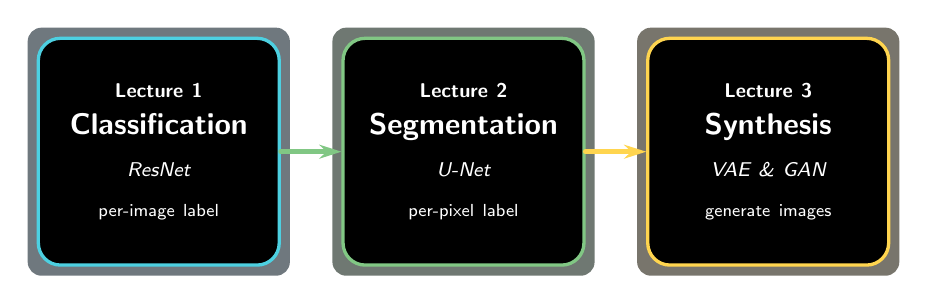
\begin{tikzpicture}[
    scale=0.9, transform shape,
    font=\sffamily\color{white},
    lecbox/.style={
        rectangle, rounded corners=8pt, draw, very thick,
        minimum width=3.4cm, minimum height=3.2cm,
        align=center, fill=black, text width=3.1cm, inner sep=4pt, text=white
    },
    mainarrow/.style={-{Stealth[length=8pt, width=5pt]}, line width=1.8pt, line cap=round}
]
\begin{scope}[on background layer]
    \node[rounded corners=5pt, minimum width=3.7cm, minimum height=3.5cm, fill=bgTeal, fill opacity=0.6] at (0,0) {};
    \node[rounded corners=5pt, minimum width=3.7cm, minimum height=3.5cm, fill=bgGreen, fill opacity=0.6] at (4.3,0) {};
    \node[rounded corners=5pt, minimum width=3.7cm, minimum height=3.5cm, fill=bgAmber, fill opacity=0.6] at (8.6,0) {};
\end{scope}

\node[lecbox, draw=accTeal]  (l1) at (0,0)   {{\footnotesize\bfseries Lecture 1}\\[0.3em] \textbf{\large Classification}\\[0.5em] {\footnotesize\itshape\color{white!75} ResNet}\\[0.4em] {\scriptsize per-image label}};
\node[lecbox, draw=accGreen] (l2) at (4.3,0) {{\footnotesize\bfseries Lecture 2}\\[0.3em] \textbf{\large Segmentation}\\[0.5em] {\footnotesize\itshape\color{white!75} U-Net}\\[0.4em] {\scriptsize per-pixel label}};
\node[lecbox, draw=accAmber] (l3) at (8.6,0) {{\footnotesize\bfseries Lecture 3}\\[0.3em] \textbf{\large Synthesis}\\[0.5em] {\footnotesize\itshape\color{white!75} VAE \& GAN}\\[0.4em] {\scriptsize generate images}};

\draw[mainarrow, accGreen] (l1) -- (l2);
\draw[mainarrow, accAmber] (l2) -- (l3);
\end{tikzpicture}

\vfill
{\footnotesize \textcolor{gray!55}{All three share one recipe --- only the model, loss, and metric change.}}
\end{frame}

%%%%%%%%%%%%%%%%%%%%%%%%%%%%%%%%%%%%%%%%%%%%%%%%
\begin{frame}{The Universal Training Recipe}
\small
\centering

{\textcolor{gray!60}{Every lecture in this module is the same loop --- swap in a task-specific
\textcolor{accTeal}{model}, \textcolor{accAmber}{loss}, and \textcolor{accGreen}{metric}.}}

\vspace{0.7cm}

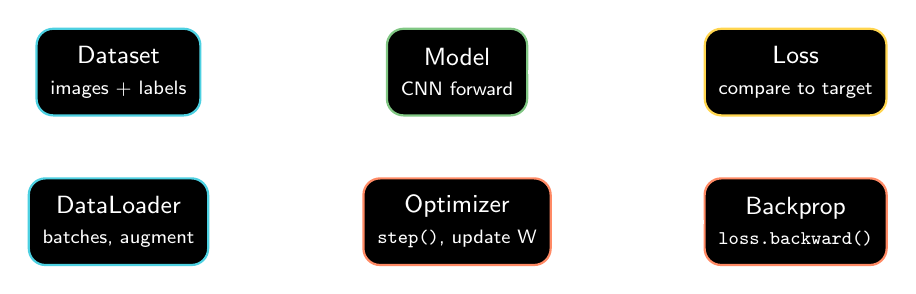
\begin{tikzpicture}[
    font=\sffamily\small\color{white},
    stepbox/.style={rectangle, rounded corners=6pt, draw, thick, minimum height=1.1cm,
        align=center, fill=black, text=white, inner sep=5pt},
    arr/.style={-{Stealth[length=7pt, width=4pt]}, line width=1.4pt, white!80}
]
\node[stepbox, draw=accTeal]  (data)  at (0,0)      {Dataset\\{\scriptsize\color{white!70}images + labels}};
\node[stepbox, draw=accTeal]  (load)  at (0,-1.9)   {DataLoader\\{\scriptsize\color{white!70}batches, augment}};
\node[stepbox, draw=accGreen] (model) at (4.3,0)    {Model\\{\scriptsize\color{white!70}CNN forward}};
\node[stepbox, draw=accAmber] (loss)  at (8.6,0)    {Loss\\{\scriptsize\color{white!70}compare to target}};
\node[stepbox, draw=accCoral] (back)  at (8.6,-1.9) {Backprop\\{\scriptsize\color{white!70}\texttt{loss.backward()}}};
\node[stepbox, draw=accCoral] (opt)   at (4.3,-1.9) {Optimizer\\{\scriptsize\color{white!70}\texttt{step()}, update W}};

\draw[arr] (load) -- (model);
\draw[arr] (model) -- (loss);
\draw[arr] (loss) -- (back);
\draw[arr] (back) -- (opt);
\draw[arr] (opt) -- (model);
\draw[arr] (data) -- (load);
\end{tikzpicture}

\vspace{0.7cm}
\begin{tcolorbox}[medicalglass, title=\textbf{What changes per task}, width=0.92\linewidth]
\begin{tabular}{@{}p{2.6cm}p{2.6cm}p{2.6cm}p{2.6cm}@{}}
 & \textcolor{accTeal}{Classification} & \textcolor{accGreen}{Segmentation} & \textcolor{accAmber}{Synthesis}\\[2pt]
\textbf{Model} & ResNet & U-Net & VAE / GAN\\
\textbf{Loss}  & Cross-entropy & Dice / CE & MSE\,+\,KL / adversarial\\
\textbf{Metric}& Accuracy, AUC & Dice, IoU & FID, visual\\
\end{tabular}
\end{tcolorbox}
\end{frame}


%%%%%%%%%%%%%%%%%%%%%%%%%%%%%%%%%%%%%%%%%%%%%%%%
%%%%%%%%%%%%%%%%%%%%%%%%%%%%%%%%%%%%%%%%%%%%%%%%
\makepart{Lecture 1: Classification --- ResNet}
%%%%%%%%%%%%%%%%%%%%%%%%%%%%%%%%%%%%%%%%%%%%%%%%

% ---- Frame 1: Bridge / recap from Module 1 ----
\begin{frame}{Recap: where Module 1 left off}
\small
\begin{columns}[c,onlytextwidth]
    \column{0.55\linewidth}
    We ended Module~1 with a classifier that maps an image to a score vector, then to
    class probabilities:
    \[
    s = f(x_i; W)
    \qquad
    P(Y{=}k \mid x_i) = \frac{e^{s_k}}{\sum_j e^{s_j}}
    \]
    \[
    L_i = -\log P(Y{=}y_i \mid x_i)
    \quad\text{\scriptsize(cross-entropy)}
    \]

    \vspace{0.6em}
    \begin{tcolorbox}[medicalglass, title=\textbf{\color{accTeal}The open question}]
    We defined the \alert{loss}. But \emph{which} function $f$? And how do we \alert{learn $W$}
    for a \textbf{deep} network?
    \end{tcolorbox}

    \column{0.42\linewidth}
    \centering
    \textbf{\footnotesize This lecture}
    \begin{itemize}\small
        \item[$\rightarrow$] $f$ = a deep \textbf{CNN}
        \item[$\rightarrow$] the block that made depth work: \alert{ResNet}
        \item[$\rightarrow$] train + evaluate it on real medical images
    \end{itemize}
\end{columns}
\end{frame}

% ---- Frame 2: Why deeper, and the degradation problem ----
\begin{frame}{Deeper should be better --- but plain nets get worse}
\small
\begin{columns}[c,onlytextwidth]
    \column{0.46\linewidth}
    \begin{itemize}\setlength\itemsep{0.5em}
        \item More layers $\Rightarrow$ richer features (Module~1: edges $\to$ parts $\to$ objects).
        \item \alert{Degradation:} beyond a point, adding layers \emph{increases} \textbf{training}
              error --- not overfitting, an \textbf{optimization} problem.
        \item A deep plain net struggles to even represent the identity mapping.
    \end{itemize}
    \vspace{0.5em}
    \begin{tcolorbox}[medicalglass, title=\textbf{\color{accCoral}The idea}]
    Let each block learn a \alert{residual} correction $F(x)$ on top of its input $x$,
    instead of a full new mapping.
    \end{tcolorbox}

    \column{0.5\linewidth}
    \centering
    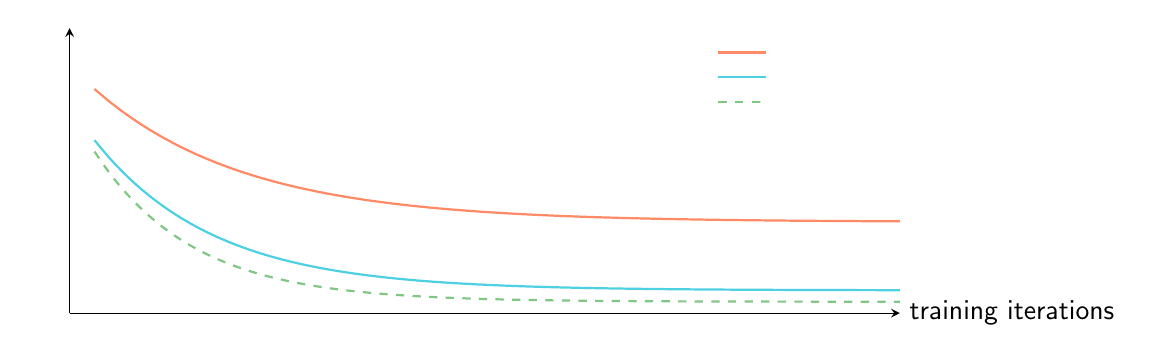
\begin{tikzpicture}
    \begin{axis}[
        width=\linewidth, height=5.2cm,
        xlabel={training iterations}, ylabel={training error},
        label style={font=\scriptsize, color=white},
        tick label style={font=\tiny, color=white},
        axis lines=left,
        every axis x label/.style={at={(ticklabel* cs:1.0)}, anchor=west},
        xmin=0, xmax=10, ymin=0, ymax=10,
        xtick=\empty, ytick=\empty,
        legend style={font=\tiny, draw=none, fill=none, text=white, at={(0.98,0.98)}, anchor=north east},
    ]
    \addplot[thick, accCoral, smooth, domain=0.3:10, samples=60] {3.2 + 5.5*exp(-0.55*x)};
    \addlegendentry{56-layer plain}
    \addplot[thick, accTeal, smooth, domain=0.3:10, samples=60] {0.8 + 6.5*exp(-0.7*x)};
    \addlegendentry{20-layer plain}
    \addplot[thick, accGreen, dashed, smooth, domain=0.3:10, samples=60] {0.4 + 6.8*exp(-0.85*x)};
    \addlegendentry{56-layer ResNet}
    \end{axis}
    \end{tikzpicture}
    \\[0.2em]
    {\tiny \color{gray!55} Illustrative --- cf. He et al., 2016}
\end{columns}
\end{frame}

% ---- Frame 3: Residual block (signature TikZ) ----
\begin{frame}{The Residual Block}
\small
\begin{columns}[c,onlytextwidth]
    \column{0.42\linewidth}
    A block computes
    \[
    y = \mathcal{F}(x, W) + x
    \]
    \begin{itemize}\setlength\itemsep{0.4em}
        \item The \alert{skip connection} adds the input back.
        \item If the ideal map is close to identity, the net just drives $\mathcal{F}\to 0$
              --- easy to learn.
        \item Gradients flow through the skip $\Rightarrow$ no vanishing in very deep nets.
    \end{itemize}

    \column{0.55\linewidth}
    \centering
    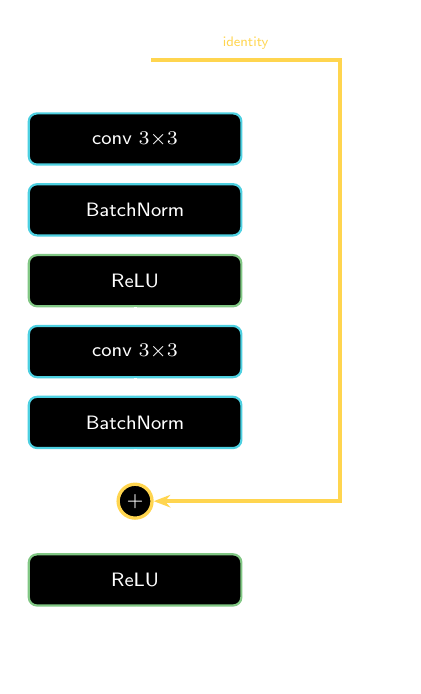
\begin{tikzpicture}[
        font=\scriptsize\sffamily\color{white},
        lyr/.style={rectangle, rounded corners=3pt, draw, thick, minimum width=2.7cm,
            minimum height=0.65cm, align=center, fill=black, text=white},
        arr/.style={-{Stealth[length=6pt]}, line width=1.1pt, white!85}
    ]
    \node (x)    at (0,0)     {$x$};
    \node[lyr, draw=accTeal]  (c1) at (0,-1.0) {conv $3{\times}3$};
    \node[lyr, draw=accTeal]  (b1) at (0,-1.9) {BatchNorm};
    \node[lyr, draw=accGreen] (r1) at (0,-2.8) {ReLU};
    \node[lyr, draw=accTeal]  (c2) at (0,-3.7) {conv $3{\times}3$};
    \node[lyr, draw=accTeal]  (b2) at (0,-4.6) {BatchNorm};
    \node[circle, draw=accAmber, very thick, fill=black, inner sep=1.5pt] (add) at (0,-5.6) {$+$};
    \node[lyr, draw=accGreen] (r2) at (0,-6.6) {ReLU};
    \node (y) at (0,-7.5) {$y$};

    \draw[arr] (x) -- (c1);
    \draw[arr] (c1) -- (b1);
    \draw[arr] (b1) -- (r1);
    \draw[arr] (r1) -- (c2);
    \draw[arr] (c2) -- (b2);
    \draw[arr] (b2) -- (add);
    \draw[arr] (add) -- (r2);
    \draw[arr] (r2) -- (y);

    % skip connection
    \draw[arr, accAmber, line width=1.3pt]
        (x.east) -- ++(2.4,0) node[midway, above, font=\tiny\color{accAmber}]{identity}
        |- (add.east);
    \node[align=center, font=\tiny\color{white!70}] at (2.9,-2.8) {$\mathcal{F}(x)$};
    \end{tikzpicture}
\end{columns}
\end{frame}

% ---- Frame 4: ResNet architecture ----
\begin{frame}{ResNet: a stack of residual blocks}
\small
\centering
\vspace{0.2cm}
\resizebox{\linewidth}{!}{%
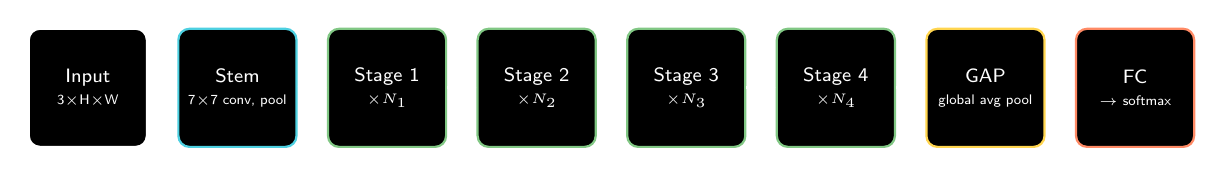
\begin{tikzpicture}[
    font=\scriptsize\sffamily\color{white},
    blk/.style={rectangle, rounded corners=4pt, draw, thick, minimum width=1.5cm,
        minimum height=1.5cm, align=center, fill=black, text=white, inner sep=2pt},
    arr/.style={-{Stealth[length=6pt]}, line width=1.2pt, white!85}
]
\node[blk, draw=white!60] (in)  at (0,0)   {Input\\{\tiny 3$\times$H$\times$W}};
\node[blk, draw=accTeal]  (stem) at (1.9,0){Stem\\{\tiny 7$\times$7 conv, pool}};
\node[blk, draw=accGreen] (s1)  at (3.8,0) {Stage 1\\{\tiny $\times N_1$}};
\node[blk, draw=accGreen] (s2)  at (5.7,0) {Stage 2\\{\tiny $\times N_2$}};
\node[blk, draw=accGreen] (s3)  at (7.6,0) {Stage 3\\{\tiny $\times N_3$}};
\node[blk, draw=accGreen] (s4)  at (9.5,0) {Stage 4\\{\tiny $\times N_4$}};
\node[blk, draw=accAmber] (gap) at (11.4,0){GAP\\{\tiny global avg pool}};
\node[blk, draw=accCoral] (fc)  at (13.3,0){FC\\{\tiny $\to$ softmax}};

\foreach \a/\b in {in/stem, stem/s1, s1/s2, s2/s3, s3/s4, s4/gap, gap/fc}
    \draw[arr] (\a) -- (\b);
\end{tikzpicture}%
}

\vspace{0.8cm}
\begin{columns}[T,onlytextwidth]
    \column{0.5\linewidth}
    \begin{tcolorbox}[medicalglass, title=\textbf{\color{accGreen}Each ``stage''}]
    A run of residual blocks at one resolution; the first block halves H$\times$W and
    doubles channels.
    \end{tcolorbox}
    \column{0.5\linewidth}
    \begin{tcolorbox}[medicalglass, title=\textbf{\color{accCoral}Depth = block counts}]
    \begin{tabular}{@{}ll@{}}
    ResNet-18 & $N=[2,2,2,2]$\\
    ResNet-34 & $N=[3,4,6,3]$\\
    ResNet-50 & bottleneck blocks
    \end{tabular}
    \end{tcolorbox}
\end{columns}
\vfill
{\tiny \color{gray!55} He, Zhang, Ren \& Sun, \emph{Deep Residual Learning for Image Recognition}, CVPR 2016.}
\end{frame}

% ---- Frame 5: The training loop, concretely ----
\begin{frame}{Training loop, concretely}
\small
\begin{columns}[c,onlytextwidth]
    \column{0.52\linewidth}
    The universal recipe, in PyTorch:
    \begin{tcolorbox}[colback=black, colframe=accTeal!60!black, coltext=white,
        arc=3pt, boxrule=1pt, fontupper=\scriptsize\ttfamily]
    for x, y in loader:\\
    \hspace*{1.5em}logits = model(x)\\
    \hspace*{1.5em}loss = criterion(logits, y)\\
    \hspace*{1.5em}optimizer.zero\_grad()\\
    \hspace*{1.5em}loss.backward()\\
    \hspace*{1.5em}optimizer.step()
    \end{tcolorbox}

    \column{0.46\linewidth}
    \begin{itemize}\setlength\itemsep{0.45em}
        \item \texttt{criterion} = \alert{CrossEntropyLoss} (softmax + NLL, from Module~1).
        \item \texttt{optimizer} = SGD(+momentum) or Adam.
        \item \texttt{zero\_grad} $\to$ \texttt{backward} $\to$ \texttt{step}: the gradient-descent
              update to $W$.
        \item One pass over the data = one \textbf{epoch}; repeat and watch val accuracy.
    \end{itemize}
\end{columns}
\vfill
{\footnotesize \textcolor{gray!55}{We run exactly this in \texttt{L1\_classification\_resnet.ipynb}.}}
\end{frame}

% ---- Frame 6: Metrics (medical framing) ----
\begin{frame}{Evaluating a classifier (medical framing)}
\small
\begin{columns}[T,onlytextwidth]
    \column{0.46\linewidth}
    \begin{tcolorbox}[medicalglass, title=\textbf{\color{accTeal}Accuracy is not enough}]
    With rare disease (Module~1 long-tail), predicting ``healthy'' can score 95\% and still
    miss every patient.
    \end{tcolorbox}
    \begin{tcolorbox}[medicalglass, title=\textbf{\color{accGreen}Confusion matrix}]
    Per-class right/wrong counts $\Rightarrow$ where the model fails.
    \end{tcolorbox}

    \column{0.5\linewidth}
    \begin{tcolorbox}[medicalglass, title=\textbf{\color{accAmber}Sensitivity / Specificity}]
    \small
    Sensitivity $=\dfrac{TP}{TP+FN}$ (catch disease)\\[0.4em]
    Specificity $=\dfrac{TN}{TN+FP}$ (avoid false alarms)
    \end{tcolorbox}
    \begin{tcolorbox}[medicalglass, title=\textbf{\color{accCoral}ROC / AUC}]
    Sweep the decision threshold; AUC summarizes the trade-off in one number.
    \end{tcolorbox}
\end{columns}
\end{frame}

% ---- Frame 7: Transfer learning ----
\begin{frame}{Transfer learning: borrow features, fine-tune}
\small
\begin{columns}[c,onlytextwidth]
    \column{0.5\linewidth}
    \begin{itemize}\setlength\itemsep{0.5em}
        \item Medical datasets are \alert{small} (Module~1: data scarcity).
        \item Start from a ResNet \textbf{pretrained on ImageNet} --- its early filters
              (edges, textures) transfer.
        \item Replace the final FC layer with one for \emph{your} classes.
        \item \textbf{Fine-tune}: train the new head (and optionally later stages) on the
              medical data.
    \end{itemize}
    \vspace{0.4em}
    {\footnotesize \textcolor{gray!55}{Often the difference between overfitting and a usable model.}}

    \column{0.48\linewidth}
    \centering
    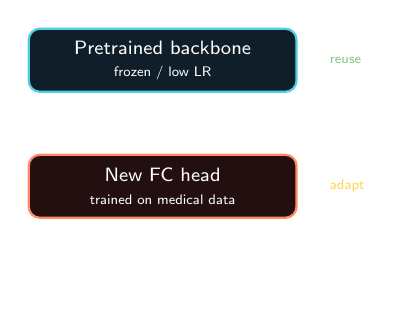
\begin{tikzpicture}[
        font=\scriptsize\sffamily\color{white},
        blk/.style={rectangle, rounded corners=4pt, draw, thick, minimum width=3.4cm,
            minimum height=0.8cm, align=center, fill=black, text=white},
        arr/.style={-{Stealth[length=6pt]}, line width=1.1pt, white!85}
    ]
    \node[blk, draw=accTeal, fill=bgTeal] (pre) at (0,0)  {Pretrained backbone\\{\tiny frozen / low LR}};
    \node[blk, draw=accCoral, fill=bgCoral] (head) at (0,-1.6) {New FC head\\{\tiny trained on medical data}};
    \node (out) at (0,-2.9) {$\to$ class probabilities};
    \draw[arr] (pre) -- (head);
    \draw[arr] (head) -- (out);
    \node[font=\tiny\color{accGreen}, align=left, anchor=west] at (2.0,0) {reuse};
    \node[font=\tiny\color{accAmber}, align=left, anchor=west] at (2.0,-1.6) {adapt};
    \end{tikzpicture}
\end{columns}
\end{frame}

% ---- Frame 8: Hands-on notebook ----
\begin{frame}{Hands-on: ResNet on PathMNIST}
\small
\begin{columns}[c,onlytextwidth]
    \column{0.52\linewidth}
    \begin{tcolorbox}[medicalglass, title=\textbf{\color{accTeal}Notebook}
        \texttt{L1\_classification\_resnet.ipynb}]
    \begin{enumerate}\small\setlength\itemsep{0.25em}
        \item \texttt{pip install medmnist}; pick GPU runtime.
        \item Load \alert{PathMNIST} (9-class digital pathology, RGB $28{\times}28$).
        \item ResNet-18: from-scratch \emph{and} pretrained + fine-tune.
        \item Train (CrossEntropy + Adam), track loss/accuracy.
        \item Evaluate: accuracy, confusion matrix, ROC/AUC.
    \end{enumerate}
    \end{tcolorbox}
    \begin{center}
    {\footnotesize \textcolor{accAmber}{$\rightarrow$ Free Colab GPU is enough; a 1-epoch smoke test runs in $<$1 min.}}
    \end{center}

    \column{0.46\linewidth}
    \centering
    \IfFileExists{Figures/pathmnist_samples.png}{%
        \includegraphics[width=\linewidth]{Figures/pathmnist_samples.png}%
    }{%
        \begin{tcolorbox}[colback=black, colframe=accTeal!60!black, coltext=white!70,
            arc=3pt, halign=center, valign=center, height=4cm, width=\linewidth]
            \footnotesize [ PathMNIST sample montage \\ exported by the notebook ]
        \end{tcolorbox}%
    }\par\vspace{0.3em}
    {\tiny \color{gray!55} PathMNIST samples (exported by the notebook). \\
    MedMNIST v2 --- Yang et al., Scientific Data 2023.}
\end{columns}
\end{frame}

% ---- Frame 9: Pitfalls ----
\begin{frame}{Pitfalls \& what to expect}
\small
\begin{columns}[T,onlytextwidth]
    \column{0.5\linewidth}
    \begin{tcolorbox}[medicalglass, title=\textbf{\color{accCoral}Overfitting}]
    Train acc $\gg$ val acc. Fixes: augmentation, weight decay, early stopping, pretrained
    weights.
    \end{tcolorbox}
    \begin{tcolorbox}[medicalglass, title=\textbf{\color{accAmber}Class imbalance}]
    Long-tailed classes get ignored. Fixes: class weights, resampling, focal loss; watch
    \emph{per-class} metrics.
    \end{tcolorbox}

    \column{0.5\linewidth}
    \begin{tcolorbox}[medicalglass, title=\textbf{\color{accTeal}Leakage}]
    Same patient in train \emph{and} test inflates accuracy. Split by \textbf{patient}, not
    by image.
    \end{tcolorbox}
    \begin{tcolorbox}[medicalglass, title=\textbf{\color{accGreen}Expect}]
    Fine-tuned ResNet-18 on PathMNIST reaches high-80s to 90s\% test accuracy in a few
    epochs.
    \end{tcolorbox}
\end{columns}
\end{frame}


%%%%%%%%%%%%%%%%%%%%%%%%%%%%%%%%%%%%%%%%%%%%%%%%
%%%%%%%%%%%%%%%%%%%%%%%%%%%%%%%%%%%%%%%%%%%%%%%%
\makepart{Lecture 2: Segmentation --- U-Net}
%%%%%%%%%%%%%%%%%%%%%%%%%%%%%%%%%%%%%%%%%%%%%%%%

% ---- L2.1 Classification -> Segmentation ----
\begin{frame}{Classification $\to$ Segmentation}
\small
\begin{columns}[c,onlytextwidth]
    \column{0.52\linewidth}
    \begin{itemize}\setlength\itemsep{0.5em}
        \item Classification: \textbf{one label per image} (``tumor present'').
        \item Segmentation: \alert{one label per pixel} (``\emph{which} pixels are tumor'').
        \item Output is a \textbf{mask} the size of the image --- delineation, volume,
              boundaries (Module~1 segmentation task).
    \end{itemize}
    \vspace{0.4em}
    \begin{tcolorbox}[medicalglass, title=\textbf{\color{accGreen}Consequence}]
    We must \emph{recover} spatial resolution after the CNN downsamples --- an
    \alert{encoder--decoder}.
    \end{tcolorbox}

    \column{0.46\linewidth}
    \centering
    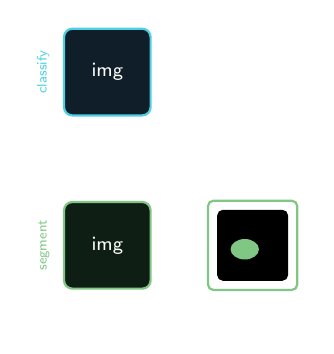
\begin{tikzpicture}[font=\scriptsize\sffamily\color{white}]
        % classification: image -> single label
        \node[draw=accTeal, thick, rounded corners=3pt, fill=bgTeal, minimum size=1.1cm] (im1) at (0,0) {img};
        \node[right=0.7cm of im1] (lab) {\textbf{``tumor''}};
        \draw[-{Stealth[length=5pt]}, white!85] (im1) -- (lab);
        \node[left=0.05cm of im1, font=\tiny\color{accTeal}, rotate=90, anchor=south] {classify};
        % segmentation: image -> mask
        \node[draw=accGreen, thick, rounded corners=3pt, fill=bgGreen, minimum size=1.1cm] (im2) at (0,-2.2) {img};
        \node[right=0.7cm of im2, draw=accGreen, thick, rounded corners=2pt, minimum size=1.1cm] (msk)
            {\tikz{\fill[black] (0,0) rectangle (0.9,0.9); \fill[accGreen] (0.35,0.4) ellipse (0.18 and 0.13);}};
        \draw[-{Stealth[length=5pt]}, white!85] (im2) -- (msk);
        \node[left=0.05cm of im2, font=\tiny\color{accGreen}, rotate=90, anchor=south] {segment};
        \node[below=0.05cm of msk, font=\tiny\color{white!70}] {per-pixel mask};
    \end{tikzpicture}
\end{columns}
\end{frame}

% ---- L2.2 The resolution problem ----
\begin{frame}{The resolution problem}
\small
\begin{columns}[c,onlytextwidth]
    \column{0.44\linewidth}
    \begin{itemize}\setlength\itemsep{0.5em}
        \item A CNN \alert{downsamples} to build semantic features --- great for \emph{what},
              but it throws away \emph{where}.
        \item Segmentation needs a \textbf{full-resolution} output.
        \item Solution: downsample to understand, then \alert{upsample} back to pixel space
              --- an \textbf{encoder--decoder}.
    \end{itemize}

    \column{0.54\linewidth}
    \centering
    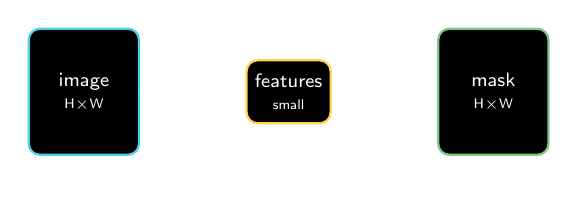
\begin{tikzpicture}[
        font=\scriptsize\sffamily\color{white},
        b/.style={rectangle, rounded corners=4pt, draw, thick, fill=black, align=center,
            text=white, inner sep=3pt},
        arr/.style={-{Stealth[length=6pt]}, line width=1.1pt, white!85}
    ]
    \node[b, draw=accTeal, minimum height=1.6cm, minimum width=1.4cm] (img) at (0,0) {image\\{\tiny H$\times$W}};
    \node[b, draw=accAmber, minimum height=0.8cm, minimum width=1.0cm] (feat) at (2.6,0) {features\\{\tiny small}};
    \node[b, draw=accGreen, minimum height=1.6cm, minimum width=1.4cm] (mask) at (5.2,0) {mask\\{\tiny H$\times$W}};
    \draw[arr] (img) -- node[above, font=\tiny\color{accTeal}]{encode} node[below, font=\tiny\color{white!60}]{downsample} (feat);
    \draw[arr] (feat) -- node[above, font=\tiny\color{accGreen}]{decode} node[below, font=\tiny\color{white!60}]{upsample} (mask);
    \node[below=0.4cm of feat, font=\tiny\color{white!70}, align=center] {\emph{what} is here};
    \end{tikzpicture}
\end{columns}
\end{frame}

% ---- L2.3 The U-Net (signature diagram) ----
\begin{frame}{The U-Net}
\small
\centering
\vspace{0.1cm}
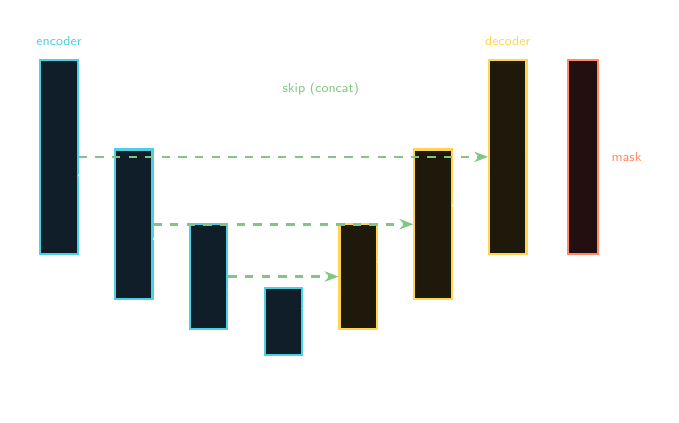
\begin{tikzpicture}[
    font=\tiny\sffamily\color{white}, scale=0.95, transform shape,
    enc/.style={rectangle, draw, thick, fill=bgTeal, draw=accTeal, minimum width=0.5cm},
    dec/.style={rectangle, draw, thick, fill=bgAmber, draw=accAmber, minimum width=0.5cm},
    arr/.style={-{Stealth[length=5pt]}, line width=1pt, white!85},
    skip/.style={-{Stealth[length=5pt]}, line width=1pt, accGreen, dashed}
]
\node[enc, minimum height=2.6cm] (e1) at (0,0)      {};
\node[enc, minimum height=2.0cm] (e2) at (1.0,-0.9) {};
\node[enc, minimum height=1.4cm] (e3) at (2.0,-1.6) {};
\node[enc, minimum height=0.9cm] (b)  at (3.0,-2.2) {};
\node[dec, minimum height=1.4cm] (d3) at (4.0,-1.6) {};
\node[dec, minimum height=2.0cm] (d2) at (5.0,-0.9) {};
\node[dec, minimum height=2.6cm] (d1) at (6.0,0)    {};
\node[rectangle, draw=accCoral, thick, fill=bgCoral, minimum height=2.6cm, minimum width=0.4cm] (out) at (7.0,0) {};

\draw[arr] (e1) -- (e2); \draw[arr] (e2) -- (e3); \draw[arr] (e3) -- (b);
\draw[arr] (b) -- (d3);  \draw[arr] (d3) -- (d2); \draw[arr] (d2) -- (d1); \draw[arr] (d1) -- (out);
\draw[skip] (e1.east) -- (d1.west);
\draw[skip] (e2.east) -- (d2.west);
\draw[skip] (e3.east) -- (d3.west);

\node[below=0.15cm of b, font=\tiny\color{white!70}] {bottleneck};
\node[above=0.05cm of e1, font=\tiny\color{accTeal}] {encoder};
\node[above=0.05cm of d1, font=\tiny\color{accAmber}] {decoder};
\node[right=0.05cm of out, font=\tiny\color{accCoral}, anchor=west] {mask};
\node[font=\tiny\color{accGreen}] at (3.5,0.9) {skip (concat)};
\end{tikzpicture}

\vspace{0.5cm}
\begin{columns}[T,onlytextwidth]
    \column{0.5\linewidth}
    \begin{tcolorbox}[medicalglass, title=\textbf{\color{accTeal}Contracting path}]
    Conv + downsample: \emph{what} is in the image (context).
    \end{tcolorbox}
    \column{0.5\linewidth}
    \begin{tcolorbox}[medicalglass, title=\textbf{\color{accAmber}Expanding path + skips}]
    Upsample and \alert{concatenate} encoder features: \emph{where} it is (localization).
    \end{tcolorbox}
\end{columns}
\vfill
{\tiny \color{gray!55} Ronneberger, Fischer \& Brox, \emph{U-Net}, MICCAI 2015.}
\end{frame}

% ---- L2.4 Upsampling + skip connections ----
\begin{frame}{Upsampling \& skip connections}
\small
\begin{columns}[c,onlytextwidth]
    \column{0.5\linewidth}
    \begin{itemize}\setlength\itemsep{0.5em}
        \item \textbf{Upsample} the coarse decoder feature (transposed conv or interpolation)
              to grow H$\times$W back.
        \item \alert{Concatenate} the matching encoder feature --- it still holds the
              \emph{fine spatial detail} lost to pooling.
        \item Result: semantics \emph{and} precise boundaries; skips also ease gradient flow.
    \end{itemize}

    \column{0.48\linewidth}
    \centering
    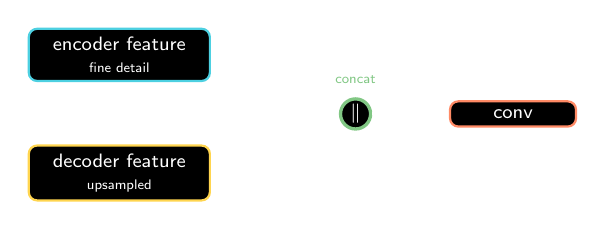
\begin{tikzpicture}[
        font=\scriptsize\sffamily\color{white},
        b/.style={rectangle, rounded corners=3pt, draw, thick, fill=black, text=white,
            align=center, inner sep=3pt, minimum width=2.3cm},
        arr/.style={-{Stealth[length=6pt]}, line width=1.1pt, white!85}
    ]
    \node[b, draw=accTeal]  (enc) at (0,0)     {encoder feature\\{\tiny fine detail}};
    \node[b, draw=accAmber] (dec) at (0,-1.5)  {decoder feature\\{\tiny upsampled}};
    \node[circle, draw=accGreen, very thick, fill=black, inner sep=1pt] (cat) at (3.0,-0.75) {\scriptsize $\Vert$};
    \node[b, draw=accCoral, minimum width=1.6cm] (conv) at (5.0,-0.75) {conv};
    \draw[arr] (enc.east) -| (cat);
    \draw[arr] (dec.east) -| (cat);
    \draw[arr] (cat) -- (conv);
    \node[above=0.05cm of cat, font=\tiny\color{accGreen}] {concat};
    \end{tikzpicture}
\end{columns}
\end{frame}

% ---- L2.5 Loss: CE vs Dice ----
\begin{frame}{Loss: cross-entropy vs.\ Dice}
\small
\begin{columns}[T,onlytextwidth]
    \column{0.5\linewidth}
    \begin{tcolorbox}[medicalglass, title=\textbf{\color{accTeal}Pixelwise cross-entropy}]
    Treat every pixel as its own classification. Simple --- but a \alert{tiny lesion} is
    swamped by background, so the net can score well by predicting ``all background''.
    \end{tcolorbox}
    \begin{tcolorbox}[medicalglass, title=\textbf{\color{accGreen}In practice}]
    Combine both: $\;\mathcal{L}=\text{BCE}+\text{Dice}$.
    \end{tcolorbox}

    \column{0.5\linewidth}
    \begin{tcolorbox}[medicalglass, title=\textbf{\color{accAmber}Dice loss}]
    Overlap-based, robust to imbalance:
    \[
    \mathcal{L}_{\text{Dice}} = 1 - \frac{2\,|P\cap G|}{|P|+|G|}
    \]
    $P$ = prediction, $G$ = ground truth. Small foreground still dominates the score.
    \end{tcolorbox}
\end{columns}
\end{frame}

% ---- L2.6 Metrics: Dice & IoU ----
\begin{frame}{Metrics: Dice \& IoU}
\small
\begin{columns}[c,onlytextwidth]
    \column{0.5\linewidth}
    \begin{tcolorbox}[medicalglass, title=\textbf{\color{accGreen}Overlap metrics}]
    \[
    \text{Dice}=\frac{2|P\cap G|}{|P|+|G|}
    \qquad
    \text{IoU}=\frac{|P\cap G|}{|P\cup G|}
    \]
    Both in $[0,1]$; higher is better.
    \end{tcolorbox}
    \begin{tcolorbox}[medicalglass, title=\textbf{\color{accAmber}Boundary error}]
    Hausdorff distance catches the \emph{worst} boundary miss --- overlap metrics can look
    fine while an edge is badly off.
    \end{tcolorbox}

    \column{0.46\linewidth}
    \centering
    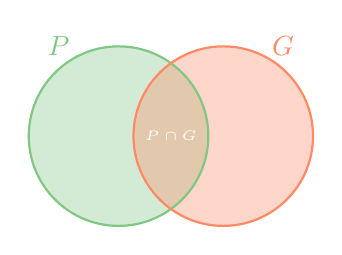
\begin{tikzpicture}[scale=0.95]
        \fill[accGreen, opacity=0.35] (0,0) circle (1.2);
        \fill[accCoral, opacity=0.35] (1.4,0) circle (1.2);
        \draw[accGreen, thick] (0,0) circle (1.2);
        \draw[accCoral, thick] (1.4,0) circle (1.2);
        \node[accGreen] at (-0.8,1.2) {$P$};
        \node[accCoral] at (2.2,1.2) {$G$};
        \node[white, font=\tiny] at (0.7,0) {$P\cap G$};
    \end{tikzpicture}
    \\[0.3em]
    {\tiny \color{gray!55} prediction $P$ vs.\ ground truth $G$}
\end{columns}
\end{frame}

% ---- L2.7 Training loop, concretely ----
\begin{frame}{Training loop, concretely}
\small
\begin{columns}[c,onlytextwidth]
    \column{0.52\linewidth}
    Same recipe as Lecture~1 --- only the \alert{model}, \alert{loss}, and \alert{output}
    change:
    \begin{tcolorbox}[colback=black, colframe=accGreen!60!black, coltext=white,
        arc=3pt, boxrule=1pt, fontupper=\scriptsize\ttfamily]
    for x, mask in loader:\\
    \hspace*{1.5em}logits = unet(x)\\
    \hspace*{1.5em}loss = bce(logits, mask)\\
    \hspace*{3.0em}+ dice\_loss(logits, mask)\\
    \hspace*{1.5em}optimizer.zero\_grad()\\
    \hspace*{1.5em}loss.backward()\\
    \hspace*{1.5em}optimizer.step()\\
    \# predict: sigmoid(logits) > 0.5
    \end{tcolorbox}

    \column{0.46\linewidth}
    \begin{itemize}\setlength\itemsep{0.45em}
        \item Model outputs a \textbf{per-pixel} logit map, not a class vector.
        \item \texttt{sigmoid} $\to$ threshold at $0.5$ gives the binary mask.
        \item Track \alert{Dice} on validation (not just loss).
        \item Heavy \textbf{augmentation} (flips, rotations, elastic) --- masks are scarce.
    \end{itemize}
\end{columns}
\end{frame}

% ---- L2.8 Hands-on ----
\begin{frame}{Hands-on: U-Net on Kvasir-SEG}
\small
\begin{columns}[c,onlytextwidth]
    \column{0.52\linewidth}
    \begin{tcolorbox}[medicalglass, title=\textbf{\color{accGreen}Notebook}
        \texttt{L2\_segmentation\_unet.ipynb}]
    \begin{enumerate}\small\setlength\itemsep{0.25em}
        \item Download \alert{Kvasir-SEG} (polyp images + masks, $\sim$46\,MB).
        \item Resize to $128{\times}128$; train/val split.
        \item U-Net from scratch (encoder--decoder + skips).
        \item Train with BCE\,+\,Dice; track \textbf{val Dice}.
        \item Overlay predicted vs.\ ground-truth masks.
    \end{enumerate}
    \end{tcolorbox}
    \begin{center}
    {\footnotesize \textcolor{accAmber}{$\rightarrow$ Free Colab GPU; \texttt{QUICK\_RUN} smoke test runs in $\sim$1 min.}}
    \end{center}

    \column{0.46\linewidth}
    \centering
    \IfFileExists{Figures/kvasir_overlay.png}{%
        \includegraphics[width=\linewidth]{Figures/kvasir_overlay.png}%
    }{%
        \begin{tcolorbox}[colback=black, colframe=accGreen!60!black, coltext=white!70,
            arc=3pt, halign=center, valign=center, height=4cm, width=\linewidth]
            \footnotesize [ image | GT mask | prediction \\ exported by the notebook ]
        \end{tcolorbox}%
    }\par\vspace{0.3em}
    {\tiny \color{gray!55} Kvasir-SEG overlay (exported by the notebook).}
\end{columns}
\end{frame}

% ---- L2.9 Pitfalls ----
\begin{frame}{Pitfalls \& what to expect}
\small
\begin{columns}[T,onlytextwidth]
    \column{0.5\linewidth}
    \begin{tcolorbox}[medicalglass, title=\textbf{\color{accCoral}Class imbalance}]
    Tiny foreground $\Rightarrow$ plain CE collapses to background. Use \textbf{Dice}
    (or combined) loss.
    \end{tcolorbox}
    \begin{tcolorbox}[medicalglass, title=\textbf{\color{accAmber}Boundaries}]
    Overlap can look good while edges leak. Watch \textbf{Hausdorff}; consider boundary
    loss.
    \end{tcolorbox}

    \column{0.5\linewidth}
    \begin{tcolorbox}[medicalglass, title=\textbf{\color{accTeal}Small data}]
    Few annotated masks $\Rightarrow$ heavy augmentation; patient-level split to avoid
    leakage.
    \end{tcolorbox}
    \begin{tcolorbox}[medicalglass, title=\textbf{\color{accGreen}Expect}]
    A from-scratch U-Net reaches \textbf{Dice $\approx$ 0.8--0.9} on Kvasir polyps within
    a few epochs.
    \end{tcolorbox}
\end{columns}
\end{frame}


%%%%%%%%%%%%%%%%%%%%%%%%%%%%%%%%%%%%%%%%%%%%%%%%
%%%%%%%%%%%%%%%%%%%%%%%%%%%%%%%%%%%%%%%%%%%%%%%%
\makepart{Lecture 3: Synthesis --- VAE \& GAN}
%%%%%%%%%%%%%%%%%%%%%%%%%%%%%%%%%%%%%%%%%%%%%%%%

% ---- L3.1 Why synthesize ----
\begin{frame}{Why synthesize medical images?}
\small
\begin{columns}[T,onlytextwidth]
    \column{0.5\linewidth}
    \begin{itemize}\setlength\itemsep{0.5em}
        \item \textbf{Augmentation:} more training data, especially \alert{rare cases}
              (Module~1 long-tail).
        \item \textbf{Modality translation:} e.g.\ CT $\leftrightarrow$ MRI.
        \item \textbf{Denoising / super-resolution} (Module~1 preprocessing task).
        \item \textbf{Privacy:} share \emph{synthetic} images instead of patient data.
    \end{itemize}
    \column{0.5\linewidth}
    \begin{tcolorbox}[medicalglass, title=\textbf{\color{accAmber}Goal}]
    Learn the data distribution $p(x)$ so we can \alert{sample} new, realistic images.
    \end{tcolorbox}
\end{columns}
\end{frame}

% ---- L3.2 Generative modeling ----
\begin{frame}{Generative modeling}
\small
\begin{columns}[c,onlytextwidth]
    \column{0.5\linewidth}
    \begin{tcolorbox}[medicalglass, title=\textbf{\color{accTeal}Discriminative}]
    Learn $p(y\mid x)$ --- a decision boundary (Lectures~1--2).
    \end{tcolorbox}
    \begin{tcolorbox}[medicalglass, title=\textbf{\color{accAmber}Generative}]
    Learn $p(x)$ --- the \emph{data itself}, so we can draw new samples $x\sim p(x)$.
    \end{tcolorbox}

    \column{0.48\linewidth}
    \begin{tcolorbox}[medicalglass, title=\textbf{\color{accGreen}Two families we cover}]
    \begin{itemize}\small\setlength\itemsep{0.4em}
        \item \textbf{VAE} --- latent-variable, likelihood-based; stable.
        \item \textbf{GAN} --- implicit, adversarial; sharp.
    \end{itemize}
    \end{tcolorbox}
    {\footnotesize \textcolor{gray!55}{Both map a simple noise/latent $z$ to an image.}}
\end{columns}
\end{frame}

% ---- L3.3 VAE architecture ----
\begin{frame}{VAE: encode $\to$ latent $\to$ decode}
\small
\centering
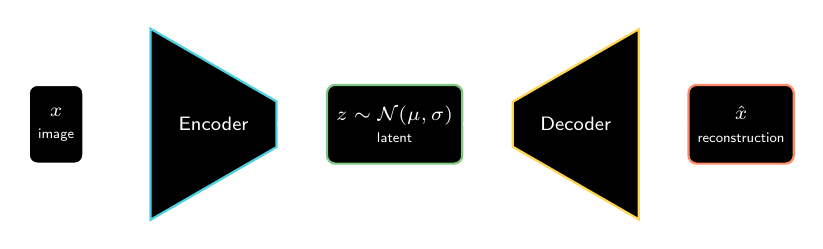
\begin{tikzpicture}[
    font=\scriptsize\sffamily\color{white},
    trap/.style={trapezium, trapezium angle=60, draw, thick, fill=black, text=white,
        minimum height=1.6cm, align=center},
    box/.style={rectangle, rounded corners=3pt, draw, thick, fill=black, text=white,
        minimum height=1.0cm, align=center},
    arr/.style={-{Stealth[length=6pt]}, line width=1.1pt, white!85}
]
\node[box, draw=white!60] (x) at (0,0) {$x$\\{\tiny image}};
\node[trap, shape border rotate=270, draw=accTeal, minimum width=1.4cm] (enc) at (2.0,0) {Encoder};
\node[box, draw=accGreen] (z) at (4.3,0) {$z \sim \mathcal{N}(\mu,\sigma)$\\{\tiny latent}};
\node[trap, shape border rotate=90, draw=accAmber, minimum width=1.4cm] (dec) at (6.6,0) {Decoder};
\node[box, draw=accCoral] (xr) at (8.7,0) {$\hat{x}$\\{\tiny reconstruction}};

\foreach \a/\b in {x/enc, enc/z, z/dec, dec/xr} \draw[arr] (\a) -- (\b);
\end{tikzpicture}

\vspace{0.6cm}
\begin{columns}[T,onlytextwidth]
    \column{0.5\linewidth}
    \begin{tcolorbox}[medicalglass, title=\textbf{\color{accTeal}Encoder}]
    Compresses $x$ into a \emph{distribution} over a low-dim latent $z$ (outputs $\mu,\sigma$).
    \end{tcolorbox}
    \column{0.5\linewidth}
    \begin{tcolorbox}[medicalglass, title=\textbf{\color{accAmber}Decoder}]
    Reconstructs an image from $z$. To \alert{generate}, sample $z\sim\mathcal{N}(0,I)$ and decode.
    \end{tcolorbox}
\end{columns}
\vfill
{\tiny \color{gray!55} Kingma \& Welling, \emph{Auto-Encoding Variational Bayes}, ICLR 2014.}
\end{frame}

% ---- L3.4 VAE loss / reparam ----
\begin{frame}{VAE: the loss (ELBO)}
\small
\begin{columns}[c,onlytextwidth]
    \column{0.5\linewidth}
    \begin{tcolorbox}[medicalglass, title=\textbf{\color{accAmber}Two terms}]
    \[
    \underbrace{\|x-\hat{x}\|^2}_{\text{recon (MSE)}}
    \;+\;
    \underbrace{\mathrm{KL}\!\big(q(z|x)\,\|\,\mathcal{N}(0,I)\big)}_{\text{regularize latent}}
    \]
    \end{tcolorbox}
    \begin{itemize}\small\setlength\itemsep{0.35em}
        \item Recon: $\hat{x}$ must look like $x$.
        \item KL: keep the latent close to $\mathcal{N}(0,I)$ so sampling is meaningful.
    \end{itemize}

    \column{0.48\linewidth}
    \begin{tcolorbox}[medicalglass, title=\textbf{\color{accTeal}Reparameterization}]
    Sampling isn't differentiable --- rewrite it:
    \[
    z=\mu+\sigma\odot\epsilon,\quad \epsilon\sim\mathcal{N}(0,I)
    \]
    Now gradients flow through $\mu,\sigma$ and we can backprop.
    \end{tcolorbox}
\end{columns}
\end{frame}

% ---- L3.5 GAN architecture ----
\begin{frame}{GAN: generator vs.\ discriminator}
\small
\centering
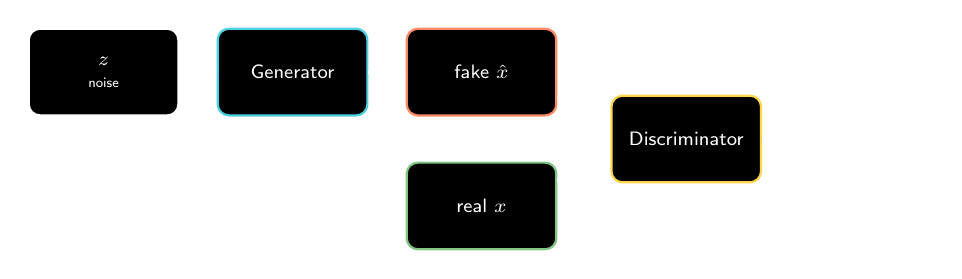
\begin{tikzpicture}[
    font=\scriptsize\sffamily\color{white},
    box/.style={rectangle, rounded corners=4pt, draw, thick, fill=black, text=white,
        minimum height=1.1cm, minimum width=1.9cm, align=center},
    arr/.style={-{Stealth[length=6pt]}, line width=1.1pt, white!85}
]
\node[box, draw=white!60] (z)  at (0,0)       {$z$\\{\tiny noise}};
\node[box, draw=accTeal]  (g)  at (2.4,0)      {Generator};
\node[box, draw=accCoral] (fake) at (4.8,0)    {fake $\hat{x}$};
\node[box, draw=accGreen] (real) at (4.8,-1.7) {real $x$};
\node[box, draw=accAmber] (d)  at (7.4,-0.85)  {Discriminator};
\node[align=left] (out) at (9.8,-0.85) {real / fake?};

\draw[arr] (z) -- (g); \draw[arr] (g) -- (fake);
\draw[arr] (fake) -- (d); \draw[arr] (real) -- (d);
\draw[arr] (d) -- (out);
\end{tikzpicture}

\vspace{0.5cm}
\begin{columns}[T,onlytextwidth]
    \column{0.5\linewidth}
    \begin{tcolorbox}[medicalglass, title=\textbf{\color{accTeal}Generator $G$}]
    Maps noise $z$ to an image; never sees real data directly --- only $D$'s feedback.
    \end{tcolorbox}
    \column{0.5\linewidth}
    \begin{tcolorbox}[medicalglass, title=\textbf{\color{accAmber}Discriminator $D$}]
    A binary classifier: real vs.\ fake. Its gradient teaches $G$.
    \end{tcolorbox}
\end{columns}
\vfill
{\tiny \color{gray!55} Goodfellow et al., \emph{Generative Adversarial Nets}, NeurIPS 2014.}
\end{frame}

% ---- L3.6 GAN training dynamics ----
\begin{frame}{GAN: the adversarial game}
\small
\begin{columns}[c,onlytextwidth]
    \column{0.52\linewidth}
    \begin{tcolorbox}[medicalglass, title=\textbf{\color{accAmber}Minimax objective}]
    \[
    \min_G \max_D \;
    \mathbb{E}[\log D(x)] + \mathbb{E}[\log(1-D(G(z)))]
    \]
    $D$ maximizes (catch fakes); $G$ minimizes (fool $D$).
    \end{tcolorbox}
    \begin{tcolorbox}[colback=black, colframe=accAmber!60!black, coltext=white,
        arc=3pt, boxrule=1pt, fontupper=\scriptsize\ttfamily]
    \# alternate each step\\
    train D: real$\to$1, fake$\to$0\\
    train G: D(fake)$\to$1  \# fool D
    \end{tcolorbox}

    \column{0.46\linewidth}
    \begin{tcolorbox}[medicalglass, title=\textbf{\color{accCoral}It's unstable}]
    \begin{itemize}\small\setlength\itemsep{0.35em}
        \item \textbf{Mode collapse:} $G$ outputs one ``safe'' image.
        \item $D$ too strong $\Rightarrow$ $G$'s gradient vanishes.
    \end{itemize}
    {\scriptsize Tricks: balanced LR, label smoothing, normalization, WGAN-GP.}
    \end{tcolorbox}
\end{columns}
\end{frame}

% ---- L3.7 VAE vs GAN ----
\begin{frame}{VAE vs.\ GAN}
\small
\centering
\vspace{0.2cm}
\begin{tcolorbox}[medicalglass, width=0.95\linewidth]
\renewcommand{\arraystretch}{1.4}
\begin{tabular}{@{}p{3.2cm}p{3.2cm}p{3.2cm}@{}}
 & \textcolor{accTeal}{\textbf{VAE}} & \textcolor{accAmber}{\textbf{GAN}}\\
\textbf{Training} & stable & unstable (collapse)\\
\textbf{Samples} & blurry & sharp\\
\textbf{Objective} & likelihood (ELBO) & adversarial (implicit)\\
\textbf{Latent} & explicit, structured & implicit\\
\textbf{Good for} & smooth interpolation, anomaly & realistic augmentation\\
\end{tabular}
\end{tcolorbox}

\vspace{0.4cm}
{\footnotesize \textcolor{gray!55}{Modern hybrids (VAE-GAN, diffusion) blend the two --- Module~3.}}
\end{frame}

% ---- L3.8 Hands-on ----
\begin{frame}{Hands-on: VAE \& GAN on MedMNIST}
\small
\begin{columns}[c,onlytextwidth]
    \column{0.5\linewidth}
    \begin{tcolorbox}[medicalglass, title=\textbf{\color{accAmber}Notebook}
        \texttt{L3\_synthesis\_vae\_gan.ipynb}]
    \begin{enumerate}\small\setlength\itemsep{0.25em}
        \item Load a MedMNIST set (28--32\,px).
        \item Build + train a \alert{VAE} (MSE\,+\,KL); sample a grid.
        \item Build + train a small \alert{DCGAN}; sample a grid.
        \item Compare VAE (blurry) vs.\ GAN (sharp).
    \end{enumerate}
    \end{tcolorbox}
    {\footnotesize \textcolor{accCoral}{VAE runs on free Colab; GAN is GPU-heavy $\rightarrow$ Colab Pro.}}

    \column{0.48\linewidth}
    \centering
    \IfFileExists{Figures/gan_samples.png}{%
        \includegraphics[width=\linewidth]{Figures/gan_samples.png}%
    }{%
        \IfFileExists{Figures/vae_samples.png}{%
            \includegraphics[width=\linewidth]{Figures/vae_samples.png}%
        }{%
            \begin{tcolorbox}[colback=black, colframe=accAmber!60!black, coltext=white!70,
                arc=3pt, halign=center, valign=center, height=4cm, width=\linewidth]
                \footnotesize [ generated sample grid \\ exported by the notebook ]
            \end{tcolorbox}%
        }%
    }\par\vspace{0.3em}
    {\tiny \color{gray!55} Synthetic samples (exported by the notebook).}
\end{columns}
\end{frame}

% ---- L3.9 Evaluation & pitfalls ----
\begin{frame}{Evaluation \& pitfalls}
\small
\begin{columns}[T,onlytextwidth]
    \column{0.5\linewidth}
    \begin{tcolorbox}[medicalglass, title=\textbf{\color{accGreen}Evaluation is hard}]
    \begin{itemize}\small\setlength\itemsep{0.3em}
        \item \textbf{FID}: distance between real/fake feature distributions.
        \item \textbf{Downstream:} does synthetic data improve a real task?
        \item Open problem (Module~4: evaluation challenges).
    \end{itemize}
    \end{tcolorbox}
    \column{0.5\linewidth}
    \begin{tcolorbox}[medicalglass, title=\textbf{\color{accCoral}Pitfalls}]
    \begin{itemize}\small\setlength\itemsep{0.3em}
        \item VAE: \emph{posterior collapse} (ignores $z$) $\to$ blur.
        \item GAN: \emph{mode collapse}, non-convergence.
        \item \textbf{Hallucination:} synthetic anatomy can mislead --- never diagnose on it.
    \end{itemize}
    \end{tcolorbox}
\end{columns}
\vfill
{\footnotesize \textcolor{gray!55}{Next: Module~3 --- beyond task-specific models (self-supervision, diffusion, foundation models).}}
\end{frame}

\end{document}
